\documentclass[11pt]{article}
\usepackage[landscape,margin=0.55in]{geometry}
\usepackage{amsmath}
\usepackage{tikz}
\usetikzlibrary{arrows.meta,calc,decorations.pathmorphing,positioning}

\pagestyle{empty}

\definecolor{occupied}{HTML}{1F6F8B}
\definecolor{path}{HTML}{D9480F}
\definecolor{target}{HTML}{7C3AED}
\definecolor{gridline}{HTML}{D7DEE8}
\definecolor{softblue}{HTML}{EAF4F8}
\definecolor{softorange}{HTML}{FFF0E6}

\begin{document}

\begin{center}
{\Large Chemical-distance estimate of $d_{\min}$}\\[4pt]
{\small What is stored: pairs of Euclidean distance $r$ and shortest-path distance $\ell$ inside the largest component.}
\end{center}

\vspace{6pt}

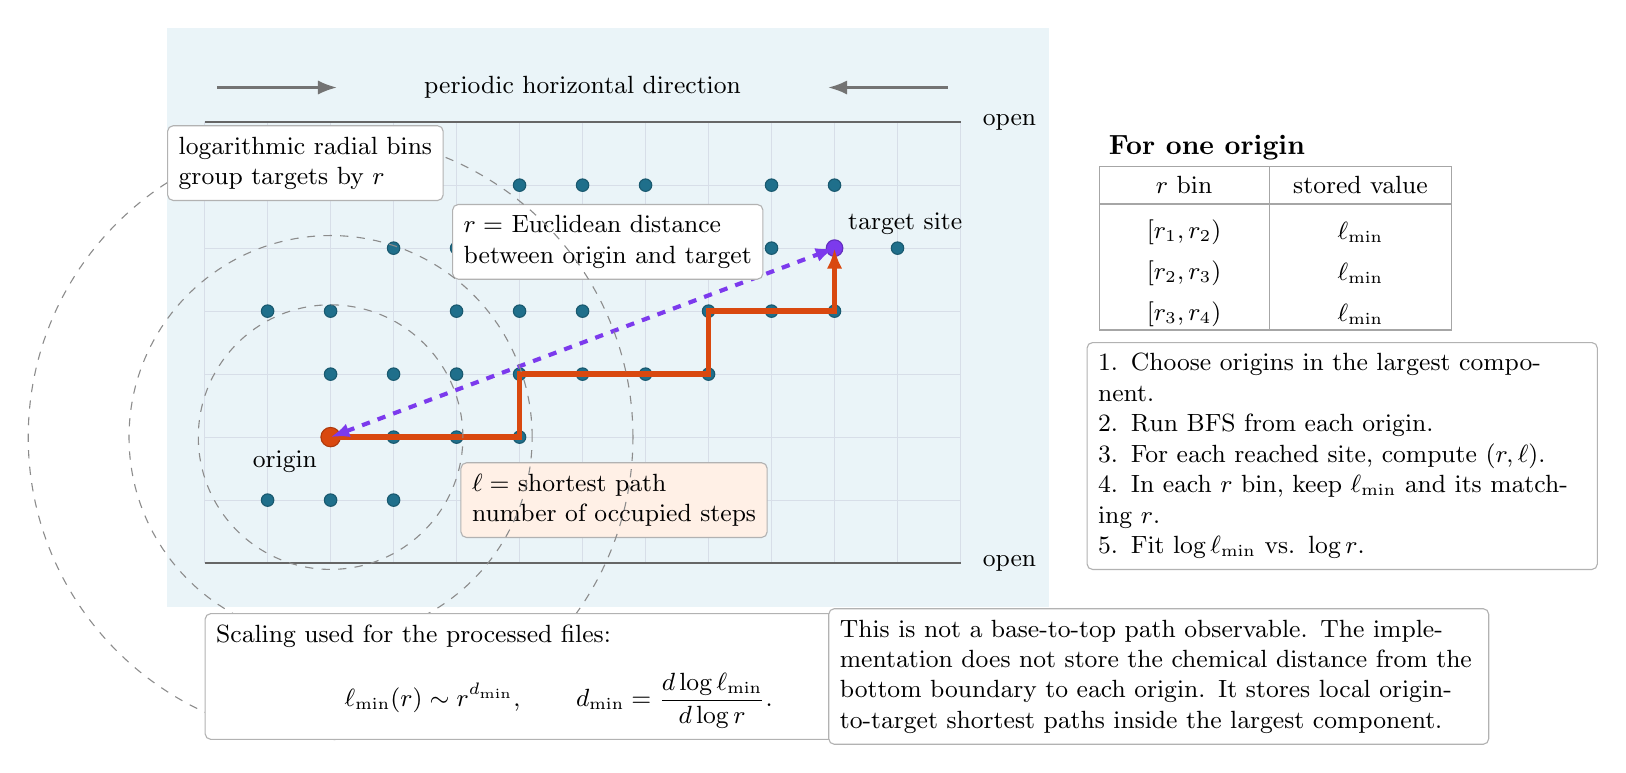
\begin{tikzpicture}[
    scale=0.80,
    every node/.style={font=\small},
    occupiedsite/.style={circle, fill=occupied, draw=occupied!80!black, minimum size=4.5pt, inner sep=0pt},
    originsite/.style={circle, fill=path, draw=path!80!black, minimum size=7pt, inner sep=0pt},
    targetsite/.style={circle, fill=target, draw=target!80!black, minimum size=6pt, inner sep=0pt},
    boxlabel/.style={draw=black!30, fill=white, rounded corners=2pt, inner sep=4pt, align=left},
    arrow/.style={-{Latex[length=2.4mm]}, thick}
]

% Panel background
\fill[softblue] (-0.6,-0.7) rectangle (13.4,8.5);

% Grid
\foreach \x in {0,...,12} {
  \draw[gridline, line width=0.25pt] (\x,0) -- (\x,7);
}
\foreach \y in {0,...,7} {
  \draw[gridline, line width=0.25pt] (0,\y) -- (12,\y);
}

% Open vertical boundaries and periodic horizontal annotation
\draw[black!60, thick] (0,0) -- (12,0);
\draw[black!60, thick] (0,7) -- (12,7);
\node[anchor=west] at (12.2,0) {open};
\node[anchor=west] at (12.2,7) {open};
\draw[arrow, black!55] (0.2,7.55) -- (2.1,7.55);
\draw[arrow, black!55] (11.8,7.55) -- (9.9,7.55);
\node at (6,7.55) {periodic horizontal direction};

% Occupied cluster points
\foreach \p in {(1,1),(2,1),(3,1),(3,2),(4,2),(5,2),(5,3),(6,3),(7,3),(8,3),(8,4),(9,4),(10,4),(10,5),(11,5),
               (2,2),(2,3),(3,3),(4,3),(4,4),(5,4),(6,4),(6,5),(7,5),(8,5),(9,5),(9,6),(10,6),
               (1,4),(2,4),(3,5),(4,5),(5,6),(6,6),(7,6)}
  \node[occupiedsite] at \p {};

% Origin and target
\coordinate (O) at (2,2);
\coordinate (T) at (10,5);
\node[originsite] at (O) {};
\node[targetsite] at (T) {};
\node[below left=2pt of O] {origin};
\node[above right=2pt of T] {target site};

% Chemical path along occupied sites
\draw[path, line width=2.1pt, -{Latex[length=2.6mm]}]
  (2,2) -- (3,2) -- (4,2) -- (5,2) -- (5,3) -- (6,3) -- (7,3) -- (8,3) -- (8,4) -- (9,4) -- (10,4) -- (10,5);
\node[boxlabel, fill=softorange] at (6.5,1.0) {$\ell=$ shortest path\\number of occupied steps};

% Euclidean distance
\draw[target, dashed, line width=1.5pt, {Latex[length=2.4mm]}-{Latex[length=2.4mm]}] (O) -- (T);
\node[boxlabel] at (6.4,5.1) {$r=$ Euclidean distance\\between origin and target};

% Radial bins
\foreach \rad/\lab in {2.1/{bin 1},3.2/{bin 2},4.8/{bin 3}} {
  \draw[black!45, dashed] (O) circle (\rad);
}
\node[boxlabel] at (1.6,6.35) {logarithmic radial bins\\group targets by $r$};

% Mini table
\begin{scope}[shift={(14.2,5.45)}]
  \node[anchor=west, font=\bfseries] at (0,1.15) {For one origin};
  \draw[black!35] (0,0.85) rectangle (5.6,-1.75);
  \draw[black!35] (0,0.25) -- (5.6,0.25);
  \draw[black!35] (2.7,0.85) -- (2.7,-1.75);
  \node at (1.35,0.55) {$r$ bin};
  \node at (4.15,0.55) {stored value};
  \node at (1.35,-0.20) {$[r_1,r_2)$};
  \node at (4.15,-0.20) {$\ell_{\min}$};
  \node at (1.35,-0.85) {$[r_2,r_3)$};
  \node at (4.15,-0.85) {$\ell_{\min}$};
  \node at (1.35,-1.50) {$[r_3,r_4)$};
  \node at (4.15,-1.50) {$\ell_{\min}$};
\end{scope}

% Algorithm box
\begin{scope}[shift={(14.0,1.7)}]
  \node[boxlabel, text width=6.2cm, anchor=west] at (0,0) {
    1. Choose origins in the largest component.\\
    2. Run BFS from each origin.\\
    3. For each reached site, compute $(r,\ell)$.\\
    4. In each $r$ bin, keep $\ell_{\min}$ and its matching $r$.\\
    5. Fit $\log \ell_{\min}$ vs. $\log r$.
  };
\end{scope}

% Fit relation
\node[boxlabel, text width=8.7cm, anchor=west] at (0,-1.8) {
  Scaling used for the processed files:
  \[
    \ell_{\min}(r) \sim r^{d_{\min}},
    \qquad
    d_{\min} = \frac{d\log \ell_{\min}}{d\log r}.
  \]
};

\node[boxlabel, text width=8.1cm, anchor=west] at (9.9,-1.8) {
  This is not a base-to-top path observable. The implementation does not store the
  chemical distance from the bottom boundary to each origin. It stores local
  origin-to-target shortest paths inside the largest component.
};

\end{tikzpicture}

\end{document}
